\section{Introduction}
\label{sec:intro}

Recent measurements~\cite{d0:fwtop, cdf:fwtop1, cdf:fwtop2} from the Tevatron experiments on inclusive forward-backward 
$t\bar{t}$ production asymmetry shows deviations from the standard model (SM) expectations.
The largest (3$\sigma$) deviation~\cite{cdf:fwtop2} is found to be in the region of high invariant mass
with $M_{t\bar{t}} > $ 450 GeV. Several attempts were made to explain this asymmetry~\cite{berger, Buckley, Gresham, zoltan}. 
One of the natural modes where such an asymmetry could be induced is via the appearance of Flavor 
Changing Neutral Current (FCNC) effects in the quark sector. Several extenstions of SM 
can generate these coupling at tree level~\cite{hills, others1}.

At the LHC, processes such as $u u \rightarrow t t$ via exchange of a $Z'$ boson
can be produced via FCNC and can appear naturally in Techicolor (TC2) models or in 
general theories with non-universal massive neutral vector bosons. In these models
the heavy boson couples strongly with the third generation of quarks which induces FCNC. 
Very recently a detailed study~\cite{berger} on forward-backward asymmetry predicts  
enhancement of same-sign top pair productions at the LHC via the $Z'$ boson. The study also 
provides explanation of the observed asymmetry at the Tevatron. 

This approach requires an interaction of $u-t-Z'$ with:

\begin{equation}
  \mathcal{L} = g_W \bar{u} \gamma^\mu (f_L P_L + f_R P_R)tZ'_\mu + h.c
\end{equation}

where $g_W$ is the weak coupling strength. The left-handed coupling is set to $f_L = 0$ throughout, due 
to the $B_d-\bar{B_d}$ mixing constraint~\cite{Cao}. The right-handed coupling $f_R$ is chosen to be a free parameter. 

\begin{figure}[htb]
\begin{center}
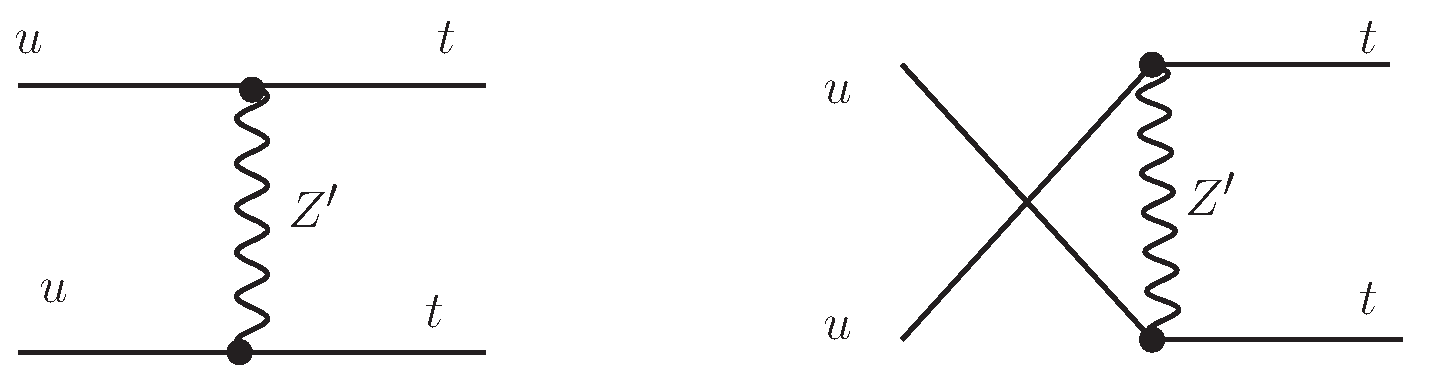
\includegraphics[width=0.7\linewidth, height=0.2\linewidth]{figs/sstop1.pdf}
\caption{ Diagrams for $tt$ pair production induced by $Z'$ exchange in t-channel. \label{fig:tchannel}}
\end{center}
\end{figure}

Fig.~\ref{fig:tchannel} shows the t-channel exchange diagrams that can lead to same-sign $tt$ final states. The initial
state involves two $u-$quarks and thus the cross section at the LHC is enhanced due to large valance quark parton 
density function (PDF). As expected the coupling appears twice in the Feynman diagrams, thus the predicated rate 
is proportional to $f_R^4$. 

\begin{figure}[htb]
\begin{center}
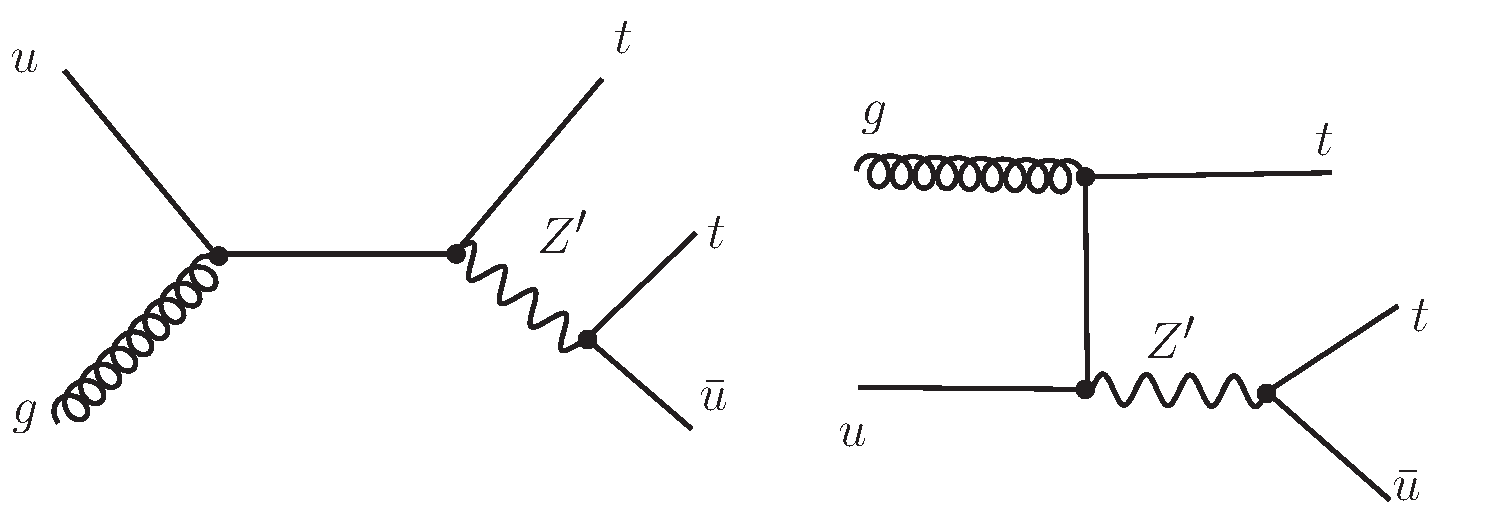
\includegraphics[width=0.7\linewidth, height=0.25\linewidth]{figs/sstop2.pdf}
\caption{ Diagrams for $tt\bar{u}$ production induced by $Z'$ exchange. \label{fig:schannel}}
\end{center}
\end{figure}

Another like sign mode is the $tt$ pair production in association with a jet, as shown 
in Fig.~\ref{fig:schannel}. The invarient mass of the $Z'$ can be recontructed using 
top quarks decay modes with an additional jet in the final state. As one of the initial parton is gluon initiated, 
we expect this rate to be lower than the t-channel diagram. We use $\alpha_Sf_R^2$ as the proportionality 
constant for the production cross section. The width of the $Z'$ boson in this case is computed using 
BRIDGE~\cite{bridge} and verified using MadGraph~\cite{madgraph}. 

\begin{figure}[htb]
\begin{center}
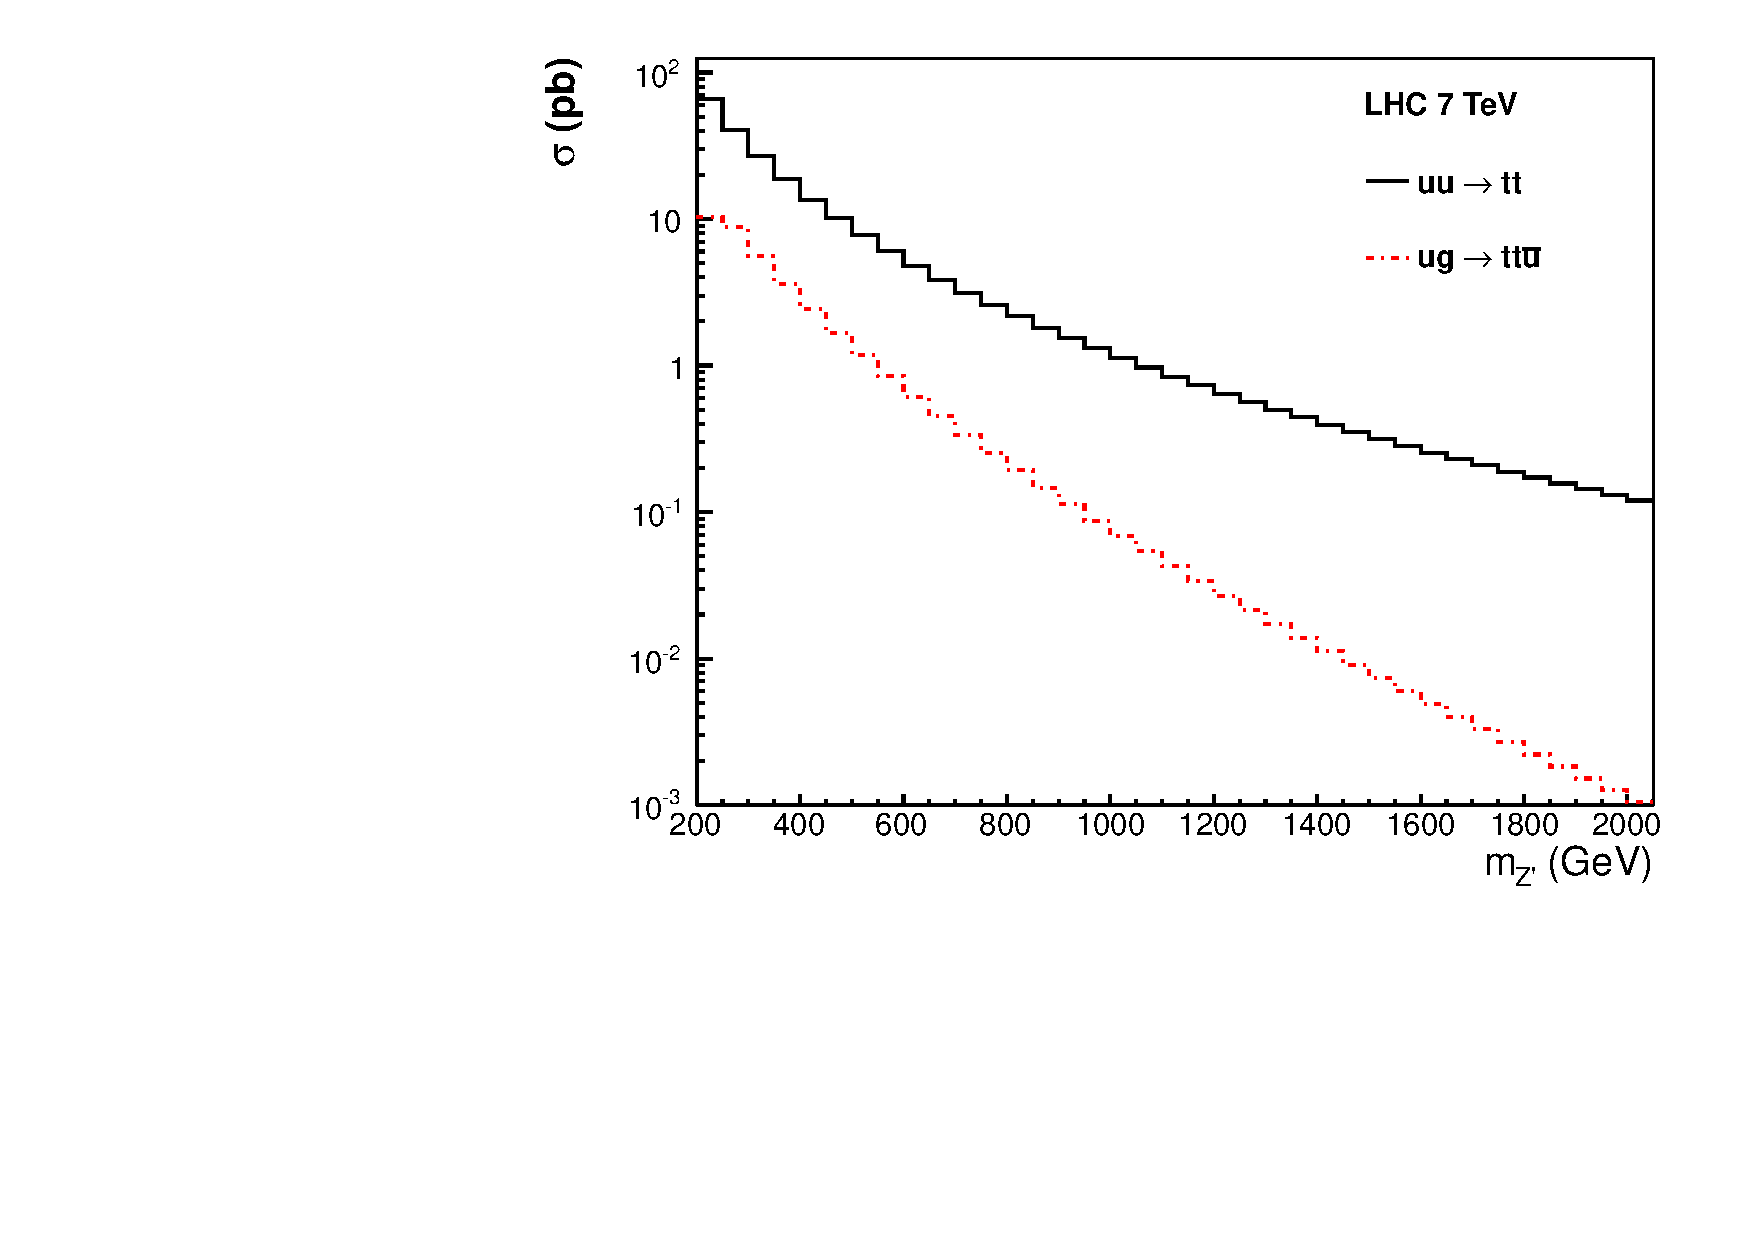
\includegraphics[width=0.7\linewidth]{figs/sstopcross.pdf}
\caption{ LHC production cross section for $tt$ and $ttj$ diagrams using right-handed coupling, $f_R = 1$. 
The renormalization and factorization scales are set to the top mass. \label{fig:sstopcross}}
\end{center}
\end{figure}

The total production cross sections at the leading-order (LO) for $tt$ and $ttj$ as a function of $Z'$ 
mass are shown in Fig.~\ref{fig:sstopcross}. The signal events are generated using the external model interface in 
MadGraph/MadEvent~\cite{madgraph}, with CTEQ6L~\cite{cteq6l} parton distribution function (PDF). The renormalization and factorization
scales are chosen to be at the top mass scale ($m_{t} = 172.5$ GeV). The cross sections agree well with the published
literature~\cite{berger}. 

In this study we search for same sign di-leptons originating from $tt$ or $ttj$ pair productions. The same sign top
production leads to $W^+ b W^+ b$ final states, where $W^+ \rightarrow l^+ \nu$. 

The note is organized as follows: in Section~\ref{sec:datasamples} we list the data samples used in this analysis; 
in Section~\ref{sec:eventselection} we describe the same sign di-lepton event selection; in Section~\ref{sec:samesign} 
we discuss the results followed by the exclusion limits in Section~\ref{sec:ssresults}. Finally, in Section~\ref{sec:conclusion} 
we summarize the results.  

The work presented here is based on previously documented studies in~\cite{ssnote1, sspaper}.

 



